\section{Mở đầu}

\subsection{Bối cảnh và vấn đề nghiên cứu}

Các ứng dụng thị giác phục vụ cảnh báo thường được tổ chức thành một chuỗi xử lý gồm
hai giai đoạn: hàm \emph{Detect} phân tích ảnh và tạo danh sách đối tượng, sau đó hàm
\emph{Alert} áp dụng luật nghiệp vụ để sinh cảnh báo. Khi chuỗi này được điều phối
trên đám mây, tổng thời gian phản hồi không chỉ phụ thuộc vào thời gian suy luận mà
còn bao gồm thời gian tải dữ liệu, gọi dịch vụ, chuyển trạng thái và truyền kết quả
giữa các hàm. Vì vậy, tối ưu riêng mô hình nhận diện chưa đủ để tối ưu độ trễ đầu
cuối của hệ thống.

Bài báo của Malazi và cộng sự chỉ ra hai giả định không còn phù hợp khi serverless
mở rộng ra môi trường Edge--Cloud--Space: trạng thái từ xa luôn đủ gần (BA6) và chi
phí chuyển giao giữa các hàm là không đáng kể (BA7)
\cite{malazi2026orchestrating}. Bài báo đồng thời đề xuất xem vị trí của trạng thái,
đường đi của dữ liệu và việc đồng vị trí các hàm là các quyết định điều phối, thay vì
coi chúng là chi tiết triển khai thứ cấp. Từ định hướng đó, nghiên cứu này khảo sát
một trường hợp cụ thể trên AWS: so sánh chuỗi \emph{Detect--Alert} được điều phối
qua AWS Step Functions với chuỗi được gọi trực tiếp trong môi trường cục bộ.

Trọng tâm của đề tài là \textbf{chi phí điều phối}, không phải độ chính xác của mô
hình thị giác. Giai đoạn Detect được sử dụng như một tải tính toán đại diện để giữ
luồng dữ liệu và giao diện giữa hai hàm giống nhau trong các kịch bản thử nghiệm.

\subsection{Mục tiêu, câu hỏi và phạm vi nghiên cứu}

Mục tiêu tổng quát của nghiên cứu là đánh giá tác động của đường điều phối đến hiệu
năng chuỗi Detect--Alert. Trên cơ sở đó, câu hỏi nghiên cứu được phát biểu như sau:

\begin{quote}
Khi giữ nguyên dữ liệu đầu vào và logic Detect--Alert, cơ chế gọi cục bộ làm thay
đổi độ trễ đầu cuối, thông lượng và lượng dữ liệu truyền qua mạng như thế nào so
với cơ chế điều phối qua AWS Step Functions?
\end{quote}

Nghiên cứu kiểm tra hai giả thuyết chính:

\begin{itemize}
    \item \textbf{H1:} Gọi cục bộ làm giảm p50 và p95 của độ trễ đầu cuối do loại
    bỏ các bước điều phối từ xa giữa Detect và Alert.
    \item \textbf{H2:} Giữ ảnh và trạng thái trung gian tại nút biên làm giảm số
    byte phải truyền qua giao diện mạng ngoài nút.
\end{itemize}

Khả năng hoạt động khi mất kết nối và mức sử dụng CPU/RAM được xem là các hướng
đánh giá tiếp theo. Hai nội dung này chưa có dữ liệu thực nghiệm Greengrass nên
không được dùng để kết luận H1 hoặc H2.

\paragraph{Mục tiêu cụ thể và phạm vi thực hiện.}
Để trả lời câu hỏi nghiên cứu, đề tài thực hiện ba nhiệm vụ:

\begin{enumerate}
    \item Xây dựng một Cloud baseline thật bằng Amazon S3, AWS Lambda, AWS Step
    Functions và Amazon CloudWatch.
    \item Xây dựng môi trường mô phỏng có kiểm soát trong đó hai kịch bản dùng cùng
    detector và logic cảnh báo, chỉ khác đường điều phối.
    \item Thu thập độ trễ, thông lượng, tỷ lệ thành công và số byte payload để đánh
    giá giả thuyết trước khi triển khai Greengrass thực tế.
\end{enumerate}

Phạm vi kết quả được phân biệt rõ như sau:

\begin{itemize}
    \item \textbf{AWS thật:} Cloud baseline đã được triển khai và hoàn thành
    1620/1620 execution qua ba mức tải 1, 3 và 5 request/s. Lambda Detect là
    container Linux ARM64 chạy YOLOv8n thật bằng PyTorch CPU.
    \item \textbf{Mô phỏng:} Edge và Cloud simulator chạy trên cùng máy phát triển
    với cùng trọng số YOLOv8n để cô lập chi phí điều phối. Đây không phải phép đo
    Greengrass.
    \item \textbf{Định hướng:} Greengrass Core, Direct Invoke giữa hai Lambda
    component là kiến trúc Edge mục tiêu; phần IPC Greengrass chưa được benchmark.
\end{itemize}

Do đó, nghiên cứu có thể đánh giá tính đúng đắn của Cloud workflow và xem kết quả
mô phỏng như bằng chứng ban đầu cho H1--H2; nghiên cứu chưa thể khẳng định mức cải
thiện trên thiết bị Greengrass thật.

\subsection{Đóng góp}

Các đóng góp có thể kiểm chứng của đề tài gồm:

\begin{enumerate}
    \item Một CloudFormation template tái tạo được Cloud baseline cùng dashboard
    giám sát.
    \item Một bộ phát tải gắn mã định danh cho từng request, theo dõi trạng thái
    Step Functions và xuất kết quả ra CSV.
    \item Một benchmark cục bộ tách độ trễ đầu cuối khỏi thời gian phục vụ, đồng
    thời báo cáo p50, p95, p99, throughput và payload mạng.
    \item Một ánh xạ cụ thể từ BA6, BA7 và IC4 của bài báo sang các quyết định về
    data locality và function chaining trong hệ thống.
\end{enumerate}


\section{Cơ sở và định hướng thiết kế}

\subsection{Chi phí điều phối và tính cục bộ dữ liệu}

Trong chuỗi Detect--Alert, đầu ra của Detect là trạng thái trung gian của Alert.
Một bộ điều phối tập trung phải tiếp nhận kết quả Detect, cập nhật trạng thái
workflow và kích hoạt Alert. Tổng độ trễ có thể biểu diễn khái quát bởi:

\begin{equation}
L_{\mathrm{E2E}} = T_{\mathrm{ingress}} + T_{\mathrm{orchestration}}
+ T_{\mathrm{detect}} + T_{\mathrm{handoff}} + T_{\mathrm{alert}}.
\label{eq:latency-components}
\end{equation}

Trong kiến trúc cục bộ, $T_{\mathrm{ingress}}$ và $T_{\mathrm{handoff}}$ không biến
mất hoàn toàn, nhưng đường đi của chúng được giới hạn trong cùng nút thực thi. Do
đó, giả thuyết của nghiên cứu là mức biến động và chi phí của hai thành phần này sẽ
nhỏ hơn so với đường đi qua dịch vụ Cloud.

\paragraph{Điều phối tập trung, choreography và gọi trực tiếp.}

Trong một workflow serverless, \emph{orchestration} là cách một thành phần trung
tâm nắm trạng thái tiến trình và quyết định hàm nào được kích hoạt tiếp theo. AWS
Step Functions thuộc mô hình này: state machine lưu tiến trình, chuyển đầu ra của
state trước thành đầu vào của state sau, đồng thời cung cấp lịch sử thực thi, retry
và xử lý lỗi. Ưu điểm là luồng điều khiển được mô tả tường minh và có thể quan sát
tập trung. Đổi lại, mọi chuyển tiếp phải đi qua mặt phẳng điều phối của dịch vụ.

\emph{Choreography} phân tán quyết định chuyển tiếp cho các thành phần tham gia,
thường thông qua sự kiện. Direct Invoke trong đề tài gần với choreography ở chỗ
Detect chủ động gọi Alert, nhưng đây vẫn là một chuỗi tuyến tính đồng bộ chứ không
phải kiến trúc hướng sự kiện đầy đủ. Nó giảm một vòng qua bộ điều phối, song làm
Detect biết giao diện của Alert và chuyển trách nhiệm retry, timeout, định danh và
ghi vết về phía ứng dụng. Vì vậy, nghiên cứu không coi Direct Invoke là phương án
tốt hơn trong mọi trường hợp. Nó phù hợp với đường cảnh báo ngắn, có quan hệ dữ
liệu chặt và yêu cầu phản hồi nhanh; Step Functions vẫn phù hợp khi workflow có
nhiều nhánh, cần bù trừ lỗi, lịch sử kiểm toán hoặc thời gian chạy dài.

Sự khác biệt này giúp xác định đúng biến độc lập của demo: thuật toán nhận diện và
luật cảnh báo được giữ nguyên, còn quyền quyết định chuyển tiếp được chuyển từ một
dịch vụ Cloud sang hàm Detect tại nút Edge. Mọi kết quả vì thế phải được diễn giải
như tác động của \emph{đường điều phối}, không phải như đánh giá tổng quát giữa hai
nền tảng có tập tính năng tương đương.

\paragraph{Ba loại trạng thái trong chuỗi Detect--Alert.}

Khái niệm ``state'' trong bài báo có thể cụ thể hóa thành ba nhóm trong demo. Thứ
nhất là \textbf{trạng thái dữ liệu}: ảnh đầu vào và danh sách bounding box. Thứ hai
là \textbf{trạng thái điều khiển}: state hiện tại, số lần thử lại và trạng thái
thành công hoặc thất bại của execution. Thứ ba là \textbf{trạng thái quan sát}:
request ID, timestamp, latency và các metric phục vụ truy vết. Cloud baseline đặt
ảnh ở S3, trạng thái điều khiển ở Step Functions và metric ở CloudWatch. Kiến trúc
Edge mục tiêu đặt dữ liệu cùng tiến trình xử lý, còn trạng thái quan sát có thể
được đệm cục bộ rồi đồng bộ lên Cloud.

Phân loại này quan trọng vì ``đưa hàm xuống Edge'' chưa đồng nghĩa với đạt data
locality. Nếu Detect chạy ở Edge nhưng phải đọc ảnh từ S3, hoặc Alert vẫn chờ một
state machine trên Cloud xác nhận, đường phụ thuộc từ xa vẫn tồn tại. Ngược lại,
việc truyền tham chiếu \texttt{bucket/key} thay cho toàn bộ ảnh trong Cloud
baseline là một tối ưu hợp lý ở tầng payload workflow, nhưng Lambda Detect vẫn
phải tải object qua mạng dịch vụ. Do đó, phép đo băng thông cuối cùng cần phân biệt
byte trong payload điều phối với byte đọc ảnh tại giao diện mạng.

\paragraph{Tính cục bộ dữ liệu theo BA6.}

BA6 mô tả sự đổ vỡ của giả định rằng trạng thái từ xa luôn có chi phí chấp nhận
được. Trong môi trường kết nối hạn chế, đọc và truyền trạng thái từ xa có thể chi
phối độ trễ và băng thông của workflow \cite{malazi2026orchestrating}. Đối với đề
tài này, ảnh là dữ liệu đầu vào có kích thước lớn, còn danh sách detection là trạng
thái trung gian nhỏ hơn. Cloud baseline lưu ảnh trên S3 và chỉ truyền tham chiếu
\texttt{bucket/key} qua Step Functions. Kiến trúc Edge mục tiêu giữ cả ảnh lẫn kết
quả detection tại nút Greengrass và chỉ đồng bộ cảnh báo hoặc telemetry khi cần.

Đề tài không xem BA6 là một kết quả đã được ``chứng minh''. BA6 được dùng để hình
thành giả thuyết H2 và quyết định đo payload mạng. Việc kiểm chứng đầy đủ cần đo
byte tại giao diện mạng của Greengrass Core thật.

\paragraph{Chi phí chuyển giao hàm theo BA7.}

BA7 đặt vấn đề rằng chi phí chuyển giao giữa các hàm thường bị xem nhẹ trong thiết
kế serverless \cite{malazi2026orchestrating}. Với Cloud baseline, chuyển giao gồm
ít nhất một lần Lambda trả kết quả về Step Functions và một lần Step Functions gọi
Lambda tiếp theo. Với kiến trúc Edge mục tiêu, Detect gọi Alert qua IPC cục bộ.
Hai hàm không chia sẻ cùng address space; chúng trao đổi một payload có cấu trúc
trên kênh IPC.

Như vậy, quyết định dùng Direct Invoke không nhằm thay đổi thuật toán Detect hoặc
Alert mà nhằm rút ngắn đường chuyển giao giữa chúng. Đây là biến độc lập chính của
thực nghiệm.

\paragraph{Tuần tự hóa, sao chép và biên thực thi.}

Mỗi lần trạng thái đi qua một biên dịch vụ, hệ thống có thể phải tuần tự hóa đối
tượng sang JSON, sao chép buffer, xác thực lời gọi và lập lịch một đơn vị thực thi
mới. Với danh sách detection nhỏ, chi phí này có thể không lớn về byte nhưng vẫn
tạo thêm latency cố định. Khi số detection hoặc metadata tăng, cả thời gian mã hóa
và kích thước payload đều tăng. Direct Invoke cục bộ không loại bỏ hoàn toàn các
chi phí này: IPC của Greengrass vẫn có biên tiến trình và payload vẫn cần định dạng
rõ ràng. Nó chỉ thay một đường chuyển tiếp qua dịch vụ từ xa bằng đường IPC trên
cùng thiết bị.

Điểm phân biệt này ngăn một diễn giải sai thường gặp: ``cục bộ'' không đồng nghĩa
với ``chia sẻ bộ nhớ''. Bản simulator truyền trực tiếp đối tượng Python nên là cận
dưới lạc quan cho chi phí handoff. Khi triển khai Greengrass thật, payload qua IPC,
chi phí runtime và cơ chế cô lập component phải được đưa vào phép đo. Chênh lệch
giữa simulator và Greengrass chính là một phần cần lượng hóa, thay vì mặc định xem
hai môi trường tương đương.

\paragraph{Cold start, warm execution và tail latency.}

AWS Lambda phân biệt giai đoạn khởi tạo môi trường thực thi với giai đoạn gọi
handler. Một môi trường mới phải chuẩn bị runtime, tải mã và chạy phần khởi tạo;
các lần gọi sau có thể tái sử dụng môi trường đã được khởi tạo
\cite{awsLambdaLifecycle}. Vì vậy, latency serverless thường không chỉ có một giá
trị trung bình mà có một phân phối gồm các lần gọi ấm nhanh hơn và một số lần gọi
lạnh chậm hơn. Trên Edge, component cũng có chi phí khởi động model; nếu component
được giữ chạy lâu dài thì chi phí này được khấu hao qua nhiều request.

Đề tài sử dụng p50 để mô tả hành vi điển hình và p95 để phản ánh phần đuôi của phân
phối. Khoảng cách lớn giữa p50 và p95 là dấu hiệu có biến động, nhưng tự nó không
chứng minh cold start. Trong thực nghiệm, cold và warm được đo riêng ngay sau khi
deploy; sau đó năm request warm-up bị loại khỏi ma trận chính. Cách này cho phép
báo cáo chi phí khởi động PyTorch mà không để nó chi phối percentile steady-state,
nhưng phần đuôi còn lại vẫn không được quy hoàn toàn cho Step Functions hay Lambda.

\subsection{Định hướng thiết kế rút ra từ bài báo}

Hai định hướng trực tiếp được rút ra từ BA6 và BA7 là giữ đường dữ liệu tại nút
Edge và rút ngắn đường chuyển giao Detect--Alert. IC4 và BA9 bổ sung góc nhìn về
vị trí trạng thái và khả năng tiếp tục xử lý khi điều phối tập trung không sẵn
sàng.

\paragraph{Các phương pháp được khai thác từ bài báo.}
Bài báo không đề xuất một thuật toán Direct Invoke cụ thể cho AWS. Thay vào đó,
nghiên cứu này khai thác bốn phương pháp thiết kế ở mức kiến trúc:

\begin{enumerate}
    \item \textbf{State-aware placement:} xem vị trí của ảnh và trạng thái detection
    là một biến thiết kế. Phương pháp này được hiện thực bằng việc giữ dữ liệu tại
    nút Edge mục tiêu, thay vì mặc định đặt state trên dịch vụ Cloud.
    \item \textbf{Composition-aware co-location:} đặt Detect và Alert trên cùng
    nút để giảm số lần state phải đi qua một dịch vụ điều phối từ xa. Trong demo,
    phương pháp này được biểu diễn bằng lời gọi trực tiếp giữa hai stage.
    \item \textbf{Local autonomy:} cho phép đường xử lý khẩn cấp hoàn tất bằng
    thông tin cục bộ, còn telemetry được đồng bộ sau. Đây là định hướng cho thử
    nghiệm mất kết nối; bản hiện tại chưa kiểm chứng thực nghiệm phương pháp này.
    \item \textbf{Telemetry-driven evaluation:} đo riêng E2E latency, stage
    latency, success rate và payload để phân biệt thời gian tính toán với chi phí
    điều phối. Cách đo này tương ứng với vai trò của telemetry agent trong kiến
    trúc ba lớp của bài báo \cite{malazi2026orchestrating}.
\end{enumerate}

Phép so sánh Cloud--Edge và cách tính percentile là phương pháp thực nghiệm do đề
tài xây dựng để lượng hóa các định hướng trên; chúng không phải kết quả hoặc quy
trình benchmark được sao chép từ bài báo.

\paragraph{IC4 và vị trí trạng thái.}

IC4 yêu cầu các nền tảng điều phối cung cấp primitive rõ ràng cho vị trí, staging,
sao chép và checkpoint trạng thái \cite{malazi2026orchestrating}. Demo áp dụng một
trường hợp đơn giản của định hướng này: trạng thái detection được đặt cùng nút với
Alert. Đây là co-location ở cấp thiết bị, không phải function-state fusion trong
cùng một tiến trình.

BA9 về điều phối tập trung được dùng làm động lực cho thí nghiệm mất kết nối trong
tương lai. Vì báo cáo chưa thực hiện thí nghiệm ngắt uplink trên Greengrass, BA9
không được xem là giả thuyết đã kiểm chứng.

\paragraph{Các bất biến của một lần thực thi.}

Bài báo tổ chức yêu cầu điều phối quanh ba nhóm bất biến: không gian--thời gian,
tài nguyên và tiến trình \cite{malazi2026orchestrating}. Trong chuỗi của đề tài,
bất biến không gian--thời gian yêu cầu Detect và Alert được đặt ở vị trí đáp ứng
ngân sách latency; bất biến tài nguyên yêu cầu nút Edge còn đủ CPU, RAM và dung
lượng lưu trữ để chạy detector; bất biến tiến trình yêu cầu một request không bị
mất hoặc xử lý sai thứ tự khi kết nối thay đổi. Ba nhóm này cho thấy việc chỉ đo
thời gian suy luận là chưa đủ để kết luận tính khả thi của một phương án Edge.

Demo hiện bao phủ bất biến không gian--thời gian ở mức mô phỏng thông qua E2E
latency và bao phủ một phần bất biến tiến trình thông qua \texttt{request\_id} và
success rate. Bất biến tài nguyên chưa được kiểm tra vì chưa có số liệu CPU, peak
RSS và dung lượng model trên Greengrass Core. Khi mở rộng thực nghiệm, một cấu hình
chỉ được coi là hợp lệ nếu đồng thời thỏa ngân sách latency, hoàn tất đủ request và
không vượt giới hạn tài nguyên. Cách đánh giá đa điều kiện này sát với lập luận của
bài báo hơn việc chỉ chọn cấu hình có latency thấp nhất.

\paragraph{Mặt phẳng điều khiển, dữ liệu và telemetry.}

Để giải thích rõ đường đi của hệ thống, có thể tách kiến trúc thành ba mặt phẳng.
Mặt phẳng dữ liệu vận chuyển ảnh và kết quả detection. Mặt phẳng điều khiển quyết
định thứ tự Detect--Alert, retry và trạng thái hoàn tất. Mặt phẳng telemetry ghi
nhận timestamp, metric, log và trạng thái tài nguyên. Trong Cloud baseline, ba mặt
phẳng này lần lượt dựa vào S3/Lambda, Step Functions và CloudWatch. Trong kiến trúc
Edge mục tiêu, hai mặt phẳng đầu hoạt động cục bộ, còn telemetry được phép đồng bộ
không đồng bộ sau khi đường cảnh báo đã hoàn tất.

CloudWatch Embedded Metric Format cho phép dịch vụ trích xuất metric từ log JSON
có cấu trúc \cite{awsCloudWatchEMF}. Demo dùng cơ chế này để phát
\texttt{DetectLatency}, \texttt{AlertLatency} và \texttt{CloudE2ELatency} mà không
cần một lời gọi API metric riêng trong đường handler. Tuy nhiên, ``quan sát được''
không có nghĩa phép đo tự động đúng: các metric so sánh phải có cùng đơn vị, cùng
khoảng thời gian và cùng statistic. Việc đặt request ID xuyên suốt ba mặt phẳng là
điều kiện để liên kết log và tránh suy luận từ các điểm dữ liệu không thuộc cùng
một request.

\paragraph{Tổng hợp ánh xạ từ bài báo sang demo.}

\begin{table}[htbp]
    \centering
    \caption{Ánh xạ luận điểm của bài báo sang thiết kế demo}
    \label{tab:paper-mapping}
    \begin{tabular}{|p{2cm}|p{5cm}|p{7cm}|}
        \hline
        \textbf{Luận điểm} & \textbf{Vấn đề} & \textbf{Cách thể hiện trong demo} \\ \hline
        BA6 & Chi phí truy cập trạng thái từ xa & So sánh luồng ảnh/payload Cloud
        với đường dữ liệu cục bộ; đo byte ở tầng ứng dụng \\ \hline
        BA7 & Chi phí handoff giữa các hàm & So sánh Step Functions handoff với
        lời gọi trực tiếp trong simulator \\ \hline
        BA9 & Điều phối tập trung phụ thuộc kết nối & Định hướng thí nghiệm ngắt
        uplink; chưa có kết quả thực nghiệm \\ \hline
        IC4 & Cần primitive cho data locality & Đặt Detect, Alert và trạng thái
        trung gian trên cùng nút Edge mục tiêu \\ \hline
    \end{tabular}
\end{table}

Từ bảng ánh xạ có thể thấy đề tài không sao chép một thuật toán có sẵn từ bài báo.
Giá trị kế thừa nằm ở cách đặt câu hỏi và lựa chọn biến đo: đường dữ liệu nằm ở
đâu, handoff đi qua bao nhiêu biên, hệ thống có tiếp tục chạy khi mất uplink hay
không, và tài nguyên tại nút có đủ để duy trì quyết định đặt hàm hay không. Demo
chuyển các câu hỏi kiến trúc đó thành một trường hợp nhỏ có thể quan sát trên AWS
Console và có thể tái chạy bằng mã nguồn.


\section{Thiết kế và hiện thực hệ thống}

\subsection{Kiến trúc đối chứng Cloud và Edge}

Hệ thống được thiết kế thành hai đường xử lý có cùng giao diện Detect--Alert nhưng
khác vị trí dữ liệu và cơ chế kích hoạt hàm kế tiếp. Cách tổ chức này giữ trọng tâm
so sánh ở đường điều phối thay vì ở thuật toán nhận diện.

\paragraph{Cloud baseline.}

Cloud baseline sử dụng đường xử lý:

\begin{center}
Load generator $\rightarrow$ S3 $\rightarrow$ Step Functions $\rightarrow$
Lambda Detect $\rightarrow$ Lambda Alert $\rightarrow$ CloudWatch.
\end{center}

Bộ phát tải tải ba đầu vào mẫu lên S3, sau đó khởi tạo một Step Functions execution
cho mỗi request. Input của state machine gồm \texttt{request\_id}, thời điểm bắt
đầu, tên bucket và object key. State \texttt{DetectObjects} gọi Lambda Detect;
\texttt{CreateAlert} nhận payload detection và gọi Lambda Alert. Alert tính độ trễ
đầu cuối rồi phát metric theo CloudWatch Embedded Metric Format.

State machine được mô tả bằng Amazon States Language và dùng tích hợp Lambda theo
mẫu request--response: state chờ lời gọi Lambda hoàn tất rồi mới chuyển sang state
kế tiếp. Với tích hợp tối ưu, Step Functions gọi Lambda và phân tích trường
\texttt{Payload} của kết quả thành JSON \cite{awsStepFunctions}. Cơ chế này tạo ra
một ranh giới đo rõ ràng giữa hai stage, đồng thời cung cấp Execution Graph và
Execution History trên AWS Console. Người trình bày có thể mở một execution để
chứng minh thứ tự \texttt{DetectObjects}--\texttt{CreateAlert}, input/output và
trạng thái thành công của từng bước.

Đường Cloud tránh đặt toàn bộ ảnh vào state machine. Payload chỉ mang
\texttt{bucket}, \texttt{key}, \texttt{request\_id} và kết quả detection cần cho
Alert. Thiết kế truyền tham chiếu này giảm kích thước trạng thái điều phối, nhưng
không loại bỏ thời gian tải ảnh từ S3 trong Detect. Do đó,
\texttt{CloudE2ELatency} là thời gian của toàn đường, trong khi Lambda Duration và
\texttt{DetectLatency} chỉ mô tả các lát cắt bên trong. Sự khác biệt về phạm vi đo
được giữ lại có chủ đích để cho thấy vì sao chỉ nhìn Duration của Lambda có thể
đánh giá thiếu chi phí hệ thống.

\begin{figure}[htbp]
    \centering
    \resizebox{\textwidth}{!}{
    \begin{tikzpicture}[
        participant/.style={
            rectangle,
            rounded corners=2pt,
            draw,
            thick,
            minimum width=2.2cm,
            minimum height=0.9cm,
            align=center,
            font=\small\bfseries
        },
        message/.style={
            -{Stealth[length=3mm]},
            thick
        },
        return/.style={
            -{Stealth[length=3mm]},
            dashed,
            thick
        },
        msglabel/.style={
            midway,
            fill=white,
            inner sep=2pt,
            font=\scriptsize
        }
    ]

    % Các thành phần
    \node[participant, fill=gray!20]   (load)   at (0,0)
        {Load\\Generator};

    \node[participant, fill=green!20]  (s3)     at (2.7,0)
        {Amazon\\S3};

    \node[participant, fill=blue!20]   (sfn)    at (5.4,0)
        {AWS Step\\Functions};

    \node[participant, fill=orange!25] (detect) at (8.1,0)
        {Lambda\\Detect};

    \node[participant, fill=orange!25] (alert)  at (10.8,0)
        {Lambda\\Alert};

    \node[participant, fill=purple!20] (cw)     at (13.5,0)
        {Amazon\\CloudWatch};

    % Lifeline
    \foreach \x in {0,2.7,5.4,8.1,10.8,13.5}
        \draw[densely dashed, gray] (\x,-0.45) -- (\x,-10.2);

    % Luồng thực thi
    \draw[message]
        (0,-1.2) --
        node[msglabel, above]{1. Upload ảnh}
        (2.7,-1.2);

    \draw[message]
        (0,-2.1) --
        node[msglabel, above]{2. StartExecution}
        (5.4,-2.1);

    \draw[message]
        (5.4,-3.0) --
        node[msglabel, above]
        {3. Invoke Detect (\texttt{bucket/key})}
        (8.1,-3.0);

    \draw[message]
        (8.1,-3.9) --
        node[msglabel, above]{4. \texttt{GetObject}}
        (2.7,-3.9);

    \draw[return]
        (2.7,-4.8) --
        node[msglabel, above]{5. Dữ liệu ảnh}
        (8.1,-4.8);

    \draw[return]
        (8.1,-5.7) --
        node[msglabel, above]
        {6. Detection payload}
        (5.4,-5.7);

    \draw[message]
        (5.4,-6.6) --
        node[msglabel, above]
        {7. Invoke Alert}
        (10.8,-6.6);

    \draw[message]
        (10.8,-7.5) --
        node[msglabel, above]
        {8. E2E và stage metrics}
        (13.5,-7.5);

    \draw[return]
        (10.8,-8.4) --
        node[msglabel, above]
        {9. Kết quả cảnh báo}
        (5.4,-8.4);

    \draw[message]
        (5.4,-9.3) --
        node[msglabel, above]
        {10. Execution logs}
        (13.5,-9.3);

    \end{tikzpicture}
    }
    \caption{Trình tự xử lý của Cloud baseline trên AWS}
    \label{fig:cloud-baseline-sequence}
\end{figure}

\paragraph{Edge mục tiêu và simulator.}

Kiến trúc mục tiêu đặt Detect và Alert trên cùng Greengrass Core. Ảnh được đọc từ
thư mục cục bộ; sau khi Detect hoàn tất, kết quả được gửi đến Alert bằng Direct
Invoke. Telemetry có thể được lưu cục bộ và đồng bộ lên Cloud sau thời điểm xử lý
khẩn cấp.

Repo hiện thực hóa đường dữ liệu này bằng \texttt{EdgeOrchestrator} trong
\texttt{edge\_demo/orchestration.py}. Đối tượng kết quả của Detect được chuyển trực
tiếp sang hàm tạo cảnh báo, không có uplink. \texttt{CloudOrchestratorSimulator}
giữ nguyên detector nhưng bổ sung tuần tự hóa và các khoảng trễ uplink, transition
và downlink cấu hình được. Nhờ vậy, phép mô phỏng chỉ khảo sát tác động của đường
điều phối; nó không tái hiện đầy đủ runtime Greengrass hoặc Step Functions.

Trong AWS IoT Greengrass V2, Lambda component được quản lý bởi các thành phần
runtime phụ trách vòng đời tiến trình và giao tiếp IPC \cite{awsGreengrassLambda}.
Vì vậy, bản triển khai mục tiêu cần đóng gói Detect và Alert thành hai component,
khai báo dependency, quyền IPC và cấu hình timeout. Detect gửi một thông điệp nhỏ
chứa detection đến Alert; ảnh gốc tiếp tục nằm trên thiết bị. Cách tổ chức này bảo
toàn ranh giới hai hàm để việc so sánh có ý nghĩa, thay vì gộp cả hai thành một hàm
Python duy nhất.

Simulator có vai trò như một \emph{controlled experiment}: các khoảng trễ mạng và
transition được khai báo rõ để kiểm tra code đo lường và chiều tác động của biến
độc lập. Greengrass có vai trò như một \emph{system experiment}: runtime, IPC,
contention CPU và I/O thật sẽ quyết định giá trị latency. Báo cáo tách hai vai trò
này để không dùng con số mô phỏng như một cam kết hiệu năng của dịch vụ AWS.

\subsection{Hiện thực chuỗi Detect--Alert và hạ tầng}

Phần hiện thực dùng một định dạng detection và một luật cảnh báo thống nhất cho cả
hai đường xử lý. Hạ tầng AWS, bộ phát tải và simulator được tổ chức thành các module
độc lập để có thể tái tạo phép đo.

\paragraph{Logic Detect--Alert.}

\texttt{edge\_demo/core.py} định nghĩa chung dữ liệu detection và logic cảnh báo.
Detector sử dụng trọng số \texttt{yolov8n.pt} tiền huấn luyện, đầu vào
$640\times640$, ngưỡng confidence 0,25 và chế độ CPU. Một cảnh báo được sinh khi
tồn tại detection có nhãn \texttt{person} và confidence không nhỏ hơn 0,60. Đầu
ra cuối là \texttt{INTRUSION\_DETECTED} hoặc \texttt{SAFE}. Model được khởi tạo
một lần ở phạm vi toàn cục và tái sử dụng giữa các invocation ấm, thay vì nạp lại
cho từng ảnh.

AWS Lambda container dùng Ultralytics 8.4.117, PyTorch 2.8.0 CPU-only và trọng số
YOLOv8n 6,55 MB. Simulator cục bộ dùng cùng phiên bản Ultralytics, PyTorch 2.8.0,
trọng số, kích thước ảnh và ngưỡng confidence. Vì tập ba ảnh không phải dataset có
nhãn, nghiên cứu chỉ xác nhận mô hình thực sự sinh detection; precision, recall và
mAP không thuộc phạm vi kết luận.

Alert là một hàm trạng thái nhẹ: nó áp dụng một predicate lên đầu ra Detect và trả
về quyết định. Việc giữ Alert thành stage riêng tạo ra handoff cần nghiên cứu và
mô phỏng đúng mô hình chuỗi hàm. Nếu chỉ quan tâm tối ưu triển khai, fusion hai
stage vào cùng tiến trình có thể còn nhanh hơn; tuy nhiên, phương án đó thay đổi
cấu trúc ứng dụng và làm mất biến đối chứng của đề tài.

\paragraph{Hạ tầng và mã nguồn.}

Các thành phần trực tiếp phục vụ thực nghiệm gồm:

\begin{table}[htbp]
    \centering
    \caption{Các tệp chính của demo}
    \label{tab:repository-files}
    \begin{tabular}{|p{6cm}|p{8cm}|}
        \hline
        \textbf{Tệp} & \textbf{Vai trò} \\ \hline
        \texttt{aws/cloudformation/template.yaml} & Tạo S3, hai Lambda, Step
        Functions, log group và CloudWatch dashboard \\ \hline
        \texttt{aws/lambda\_detect\_yolo/} & Dockerfile, handler và dependency
        cho Lambda container YOLOv8n \\ \hline
        \texttt{aws/deploy\_yolo\_cloud.sh} & Tạo ECR, build/push image ARM64 và
        cập nhật CloudFormation stack \\ \hline
        \texttt{aws/run\_cloud\_demo.py} & Tải ảnh, phát request, chờ kết quả và
        ghi CSV \\ \hline
        \texttt{edge\_demo/core.py} & Detector, cấu trúc detection và luật cảnh
        báo dùng chung \\ \hline
        \texttt{edge\_demo/orchestration.py} & Hai đường điều phối mô phỏng Cloud
        và Edge \\ \hline
        \texttt{edge\_demo/benchmark.py} & Phát tải đồng thời, tính percentile,
        throughput và xuất báo cáo \\ \hline
        \texttt{tests/test\_demo.py} & Kiểm tra request ID, network byte và khả
        năng xử lý đủ request \\ \hline
    \end{tabular}
\end{table}

CloudFormation tạo Lambda Detect dạng container ARM64 với 3008 MB RAM, 1024 MB
ephemeral storage và timeout 120 giây; Lambda Alert dùng 128 MB. Detect đọc object
S3, chạy YOLOv8n và phát \texttt{ImageDownloadLatency},
\texttt{ModelInferenceLatency} cùng \texttt{DetectLatency}. Alert phát
\texttt{AlertLatency} và \texttt{CloudE2ELatency}. Dashboard hiển thị E2E,
stage latency, model inference, số execution và Lambda Duration.

Việc mô tả hạ tầng bằng CloudFormation hỗ trợ tính tái lập: tên logic, quyền thực
thi, state machine và dashboard được tạo từ cùng một template. Stack output cung
cấp ARN của state machine, bucket và liên kết Console để bộ phát tải không cần mã
hóa cứng tài nguyên. Tuy nhiên, tái lập hạ tầng không tự động bảo đảm tái lập kết
quả. Phiên bản mã Lambda, Region, kích thước bộ nhớ, thời điểm chạy và tập ảnh vẫn
phải được ghi trong metadata của mỗi lần benchmark.

Về bảo mật, người chạy demo chỉ cần quyền triển khai stack và quyền gọi các tài
nguyên thuộc stack. Lambda Detect cần đọc object trong đúng bucket; Step Functions
chỉ cần gọi hai Lambda được chỉ định; log role chỉ cần ghi vào log group tương ứng.
Nguyên tắc đặc quyền tối thiểu vừa giảm rủi ro vừa làm rõ quan hệ phụ thuộc giữa
các thành phần. Access key không được đặt trong mã nguồn hoặc tệp kết quả; AWS CLI
nên lấy credential từ profile cục bộ và có thể thay bằng role hoặc credential tạm
thời khi triển khai lâu dài.

\subsection{Quan sát, định danh và tiêu chí hoàn tất}

Mỗi request được gắn UUID và giữ nguyên qua S3 reference, Step Functions, Detect,
Alert và CSV. Một request được coi là thành công khi Step Functions kết thúc ở trạng
thái \texttt{SUCCEEDED} và trả về đúng \texttt{request\_id}. Success rate chỉ phản
ánh tính hoàn tất của workflow, không phản ánh accuracy hoặc mAP của detector.

\paragraph{Idempotency và ngữ nghĩa thực thi.}

Trong hệ phân tán, timeout ở phía gọi không luôn đồng nghĩa với hàm chưa xử lý.
Một lần retry có thể khiến Alert nhận cùng request nhiều hơn một lần. Nếu hành động
thật là mở còi, gửi SMS hoặc ghi sự kiện bảo mật, xử lý lặp sẽ tạo tác dụng phụ.
Vì vậy, \texttt{request\_id} không chỉ phục vụ đo latency mà còn có thể làm khóa
idempotency: Alert ghi nhận ID đã xử lý và trả lại kết quả cũ khi nhận bản sao.

Demo hiện kiểm tra tính nhất quán request ID nhưng chưa cài kho chống trùng bền
vững. Trong Greengrass, có thể lưu tập ID gần nhất vào local store với thời gian
hết hạn; trong Cloud, có thể dùng một kho khóa có điều kiện. Báo cáo vì thế chỉ xác
nhận \emph{completion semantics} của lần chạy, chưa tuyên bố exactly-once. Cách
phát biểu chính xác hơn là workflow có thể được thiết kế theo at-least-once kết hợp
với Alert idempotent.

\paragraph{Khả năng quan sát đầu cuối.}

Một trace logic được hình thành từ UUID, thời điểm lên lịch, thời điểm bắt đầu xử
lý, thời điểm hoàn tất và trạng thái của từng stage. Trên AWS Console, UUID có thể
được dùng để đối chiếu execution của Step Functions với log của hai Lambda. Trong
CSV, cùng UUID liên kết E2E latency với trạng thái thành công. Trên Edge, cùng quy
ước phải được giữ trong log cục bộ để dữ liệu đồng bộ muộn vẫn ghép đúng request.

Ba dấu hiệu được dùng để kết luận một lần demo hoàn tất là: CloudFormation stack ở
trạng thái ổn định, toàn bộ Step Functions execution đã kết thúc và file CSV có đủ
số dòng request với ID duy nhất. Dashboard là bằng chứng quan sát bổ sung, không
thay thế kiểm tra completeness trong CSV vì CloudWatch có thể tổng hợp metric theo
chu kỳ và hiển thị chậm hơn thời điểm execution kết thúc.


\section{Phương pháp thực nghiệm}

\subsection{Thiết kế kịch bản và chỉ số đánh giá}

Nghiên cứu sử dụng hai nhóm dữ liệu độc lập:

\begin{enumerate}
    \item \textbf{AWS Cloud thật:} ba workload có cùng thời lượng phát tải danh
    nghĩa 180 giây được chạy ở 1, 3 và 5 request/s, tương ứng 180, 540 và 900
    request, để đánh giá khả năng duy trì độ trễ và tỷ lệ thành công khi tăng tải.
    \item \textbf{Mô phỏng có kiểm soát:} ba workload 1, 3 và 5 request/s được
    chạy cho cả Edge simulator và Cloud simulator, tương ứng 180, 540 và 900
    request trên mỗi nhánh.
\end{enumerate}

Hai nhóm không được đặt trong cùng một phép so sánh định lượng vì khác môi trường
thực thi. Kết quả AWS dùng để mô tả Cloud baseline; kết quả simulator dùng để kiểm
tra giả thuyết về đường điều phối trong điều kiện kiểm soát.

\begin{table}[htbp]
    \centering
    \caption{Cấu hình ba workload trên AWS Cloud baseline}
    \label{tab:aws-load-config}
    \begin{tabular}{|c|r|r|r|}
        \hline
        \textbf{Tải mục tiêu} & \textbf{Số request} & \textbf{Số worker}
        & \textbf{Thời lượng danh nghĩa} \\ \hline
        1 request/s & 180 & 4 & 180 giây \\ \hline
        3 request/s & 540 & 12 & 180 giây \\ \hline
        5 request/s & 900 & 20 & 180 giây \\ \hline
    \end{tabular}
\end{table}

Số worker được tăng tỷ lệ thuận với tốc độ phát để tránh hàng đợi tại máy client
trở thành nút thắt. Mỗi request sử dụng một UUID và một trong các ảnh mẫu theo thứ
tự luân phiên. Ba CSV được tổng hợp bằng cùng một hàm percentile; request không ở
trạng thái \texttt{SUCCEEDED} bị loại khỏi thống kê latency nhưng vẫn được tính
vào mẫu số của success rate.

Ba CSV lưu \texttt{scheduled\_at\_s}, \texttt{submitted\_at\_s} và
\texttt{completed\_at\_s}. Throughput quan sát đạt 0,999; 2,983 và 4,956
request/s, gần với ba tốc độ mục tiêu. Mỗi dòng còn ghi
\texttt{detector=YOLOv8n}, số detection, Detect latency và inference latency để
kiểm tra backend thực thi cho từng request.

\begin{table}[htbp]
    \centering
    \caption{Cấu hình YOLOv8n được cố định trong thực nghiệm}
    \label{tab:yolo-config}
    \begin{tabular}{|l|l|}
        \hline
        \textbf{Tham số} & \textbf{Giá trị} \\ \hline
        Trọng số & \texttt{yolov8n.pt}, 6,55 MB \\ \hline
        Runtime & Ultralytics 8.4.117; PyTorch 2.8.0 CPU-only \\ \hline
        Kích thước đầu vào & 640 pixel \\ \hline
        Ngưỡng detection & 0,25 \\ \hline
        Luật Alert & \texttt{person} với confidence $\geq 0,60$ \\ \hline
        AWS Detect & Lambda container ARM64, 3008 MB, timeout 120 giây \\ \hline
        Local simulator & macOS ARM64, CPU, warm-up 3 request/mode \\ \hline
    \end{tabular}
\end{table}

\paragraph{Mô hình tải và hàng đợi.}

Bộ phát tải đọc luân phiên các ảnh trong thư mục và lên lịch request theo tốc độ
cấu hình trước. Đây là mô hình \emph{open-loop}: thời điểm phát request mới không
phụ thuộc request trước đã hoàn tất hay chưa. Mô hình này phù hợp với camera tạo
frame theo chu kỳ và cho phép quan sát hàng đợi khi tốc độ đến vượt khả năng xử lý.
Nếu dùng closed-loop, mỗi worker chỉ gửi request tiếp theo sau khi nhận kết quả;
khi hệ thống chậm, nguồn tải cũng tự chậm lại và có thể che giấu hiện tượng quá tải.

Gọi $\lambda$ là tốc độ đến và $\mu$ là tốc độ phục vụ hiệu dụng. Khi $\lambda$
tiệm cận hoặc vượt $\mu$, thời gian chờ tăng và E2E latency có thể tăng mạnh dù
service latency của từng request gần như không đổi. Bởi vậy, demo ghi cả hai đại
lượng. Khoảng cách

\begin{equation}
T_{\mathrm{queue}}^{(i)} = L_{\mathrm{E2E}}^{(i)}
- L_{\mathrm{service}}^{(i)}
\label{eq:queue-delay}
\end{equation}

xấp xỉ thời gian request chờ trước khi được worker phục vụ. Đây không phải phép đo
hàng đợi nội bộ của AWS, mà là hàng đợi ở phía bộ phát tải. Trong ma trận thực
nghiệm hoàn chỉnh, các mức 1, 5, 10 và 20 request/s giúp xác định điểm mà latency
bắt đầu tăng nhanh hoặc success rate giảm.

\paragraph{Chỉ số và công thức đo.}

Độ trễ đầu cuối của request $i$ là:

\begin{equation}
L_{\mathrm{E2E}}^{(i)} = t_{\mathrm{completed}}^{(i)}
- t_{\mathrm{scheduled}}^{(i)}.
\label{eq:e2e-latency}
\end{equation}

Định nghĩa này bao gồm cả thời gian chờ worker khi tốc độ đầu vào vượt khả năng xử
lý. \texttt{service\_latency\_ms} chỉ đo từ lúc worker bắt đầu gọi orchestrator đến
khi lời gọi hoàn tất.

Success rate và throughput được tính bởi:

\begin{equation}
SR = \frac{N_{\mathrm{succeeded}}}{N_{\mathrm{total}}}\times 100\%,
\qquad
R = \frac{N_{\mathrm{completed}}}{T_{\mathrm{wall}}}.
\label{eq:success-throughput}
\end{equation}

Payload mạng trong simulator là số byte ứng dụng đi qua đường biên Cloud, không
bao gồm TCP/IP, TLS hoặc framing. Giá trị 0 của Edge simulator có nghĩa là không có
external payload trong mô hình này; nó không có nghĩa tiến trình không thực hiện
bất kỳ I/O nào.

Mức giảm p50 trong cùng môi trường mô phỏng được tính bởi:

\begin{equation}
G_{p50} = \frac{P_{50}^{\mathrm{cloud\_sim}}
- P_{50}^{\mathrm{edge\_sim}}}{P_{50}^{\mathrm{cloud\_sim}}}\times 100\%.
\label{eq:p50-reduction}
\end{equation}

Ngoài percentile, hệ số biến thiên có thể được dùng để so sánh mức ổn định tương
đối giữa các cấu hình:

\begin{equation}
CV = \frac{s}{\bar{x}},
\label{eq:coefficient-variation}
\end{equation}

trong đó $s$ là độ lệch chuẩn mẫu và $\bar{x}$ là latency trung bình. Tuy nhiên,
phân phối latency thường lệch phải nên median, IQR và percentile có ý nghĩa trực
quan hơn mean và standard deviation. Với $n=20$, p95 gần như do một trong những
quan sát lớn nhất quyết định; p99 hầu như không ổn định. Báo cáo vì thế chỉ dùng
p95 AWS như mô tả của lần chạy và yêu cầu tối thiểu 100 request cùng nhiều lần lặp
cho kết luận sau này.

\paragraph{Đồng hồ và biên đo.}

Độ trễ trong một tiến trình nên dùng đồng hồ đơn điệu để tránh ảnh hưởng khi đồng
hồ hệ thống được hiệu chỉnh. Với đường AWS, timestamp phải đi qua nhiều dịch vụ,
nên E2E được neo tại bộ phát tải hoặc truyền một timestamp chuẩn thống nhất. Nếu
lấy timestamp ở hai máy khác nhau, sai lệch đồng hồ có thể bị nhầm thành network
latency. Mỗi metric vì thế cần ghi rõ điểm bắt đầu và kết thúc: scheduled-to-done,
worker-start-to-done, handler-start-to-handler-end hay state-enter-to-state-exit.

Đối với CloudWatch, statistic hiển thị trên widget còn phụ thuộc period. Average
trên một bucket một phút không thể so trực tiếp với p95 của từng request trong CSV.
Để trình bày kết quả, dashboard nên chọn cùng khoảng thời gian chạy, period một
phút cho xu hướng, và dùng CSV để tính percentile đầu cuối. Execution History được
dùng xác minh một request cụ thể; dashboard dùng mô tả xu hướng toàn bộ đợt chạy.

\subsection{Kiểm soát và giới hạn phép đo}

Trong simulator, hai nhánh sử dụng cùng tập tệp, detector, ngưỡng cảnh báo, số
request và request rate. Chúng chỉ khác orchestrator. AWS Cloud và simulator không
có cùng phần cứng, runtime hoặc network nên không được xem là một cặp đối chứng.

Tập đầu vào mặc định gồm ba tệp tổng hợp phục vụ kiểm thử logic, không phải một bộ
dữ liệu thị giác có nhãn. Vì thế nghiên cứu không đo precision, recall hay mAP.

Mỗi mức tải AWS có ít nhất 180 request. Trước ma trận chính, năm invocation đồng
thời được chạy ngoài tập đo để làm ấm pool Lambda. Cold-start được đo riêng: lần
đầu sau deploy có E2E 64,41 giây, trong khi request ấm kế tiếp có E2E 1,97 giây.
Tuy vậy, mỗi cấu hình chính mới chỉ chạy một lần; benchmark hoàn chỉnh vẫn cần lặp
độc lập và luân phiên thứ tự tải.

\paragraph{Biến kiểm soát và tính công bằng.}

Để so sánh Cloud với Greengrass thật, các biến ứng dụng phải được cố định: cùng ảnh
theo cùng thứ tự, cùng phiên bản YOLOv8n, cùng trọng số, cùng kích thước đầu vào,
cùng confidence threshold và cùng luật Alert. Biến hạ tầng không thể giống hoàn
toàn, nhưng phải được mô tả: loại CPU, số vCPU, RAM, hệ điều hành, Region, Lambda
memory, kiến trúc bộ xử lý và trạng thái kết nối. Trong bộ kết quả mới, Lambda
Cloud và hai nhánh simulator đều dùng YOLOv8n thật; khác biệt phần cứng giữa AWS
Linux ARM64 và máy Mac vẫn khiến số tuyệt đối giữa hai môi trường không thể so
trực tiếp.

Thứ tự chạy cũng có thể gây sai lệch do cache và nhiệt độ thiết bị. Mỗi cấu hình
nên có pha warm-up, sau đó luân phiên thứ tự Cloud--Edge giữa các lần lặp. Tệp kết
quả cần lưu seed, run ID, thời gian UTC và cấu hình command line. Median của năm
lần lặp được dùng làm giá trị trung tâm; IQR thể hiện biến thiên giữa các lần lặp.

\paragraph{Đe dọa đối với giá trị thực nghiệm.}

Giá trị nội tại bị đe dọa nếu hai nhánh khác detector hoặc nếu độ trễ giả lập được
chọn để tạo ra kết quả mong muốn. Biện pháp giảm thiểu là dùng chung implementation
và công bố toàn bộ tham số simulator. Giá trị cấu trúc bị đe dọa khi
\texttt{network\_bytes} ở tầng ứng dụng được gọi là tổng băng thông; báo cáo tránh
điều này bằng cách mô tả đúng biên đo. Giá trị bên ngoài bị giới hạn vì VM
Greengrass không đại diện cho mọi camera hoặc thiết bị nhúng. Giá trị kết luận bị
giới hạn bởi cỡ mẫu nhỏ và thiếu khoảng tin cậy.

Các đe dọa trên không làm demo mất giá trị, nhưng giới hạn loại kết luận có thể rút
ra. Bản hiện tại chứng minh workflow chạy được và kiểm tra cơ chế đo; bản
Greengrass lặp nhiều lần mới trả lời định lượng câu hỏi nghiên cứu. Việc công khai
ranh giới bằng chứng là một phần của phương pháp khoa học, đặc biệt khi simulator
cho mức giảm lớn.


\section{Kết quả và thảo luận}

\subsection{Kết quả thực nghiệm}

Kết quả được chia thành hai nhóm bằng chứng: Cloud baseline trên AWS dùng để xác
nhận workflow thật, còn simulator dùng để khảo sát tác động của đường điều phối
trong điều kiện kiểm soát. Hai nhóm được trình bày riêng và không được xem là hai
môi trường tương đương.

\paragraph{Cloud baseline trên AWS.}

CloudFormation stack đã được cập nhật để Lambda Detect lấy image YOLOv8n từ ECR.
Ba workload phát tổng cộng 1620 Step Functions execution; mọi dòng CSV đều có
\texttt{detector=YOLOv8n} và toàn bộ kết thúc ở trạng thái
\texttt{SUCCEEDED}. Kết quả được trình bày trong Bảng~\ref{tab:aws-results}.

\begin{table}[htbp]
    \centering
    \caption{Kết quả Cloud baseline theo ba mức tải}
    \label{tab:aws-results}
    \begin{tabular}{|l|r|r|r|}
        \hline
        \textbf{Chỉ số} & \textbf{1 req/s} & \textbf{3 req/s}
        & \textbf{5 req/s} \\ \hline
        Số request & 180 & 540 & 900 \\ \hline
        Số request thành công & 180 & 540 & 900 \\ \hline
        Success rate & 100\% & 100\% & 100\% \\ \hline
        Mean E2E (ms) & 968,15 & 856,67 & 925,56 \\ \hline
        p50 E2E (ms) & 966,56 & 842,85 & 921,08 \\ \hline
        p95 E2E (ms) & 1076,56 & 978,10 & 1080,49 \\ \hline
        p99 E2E (ms) & 1155,17 & 1081,76 & 1182,76 \\ \hline
        Giá trị lớn nhất (ms) & 1293,42 & 1708,99 & 2451,32 \\ \hline
        Throughput (request/s) & 0,999 & 2,983 & 4,956 \\ \hline
    \end{tabular}
\end{table}

\begin{figure}[htbp]
    \centering
    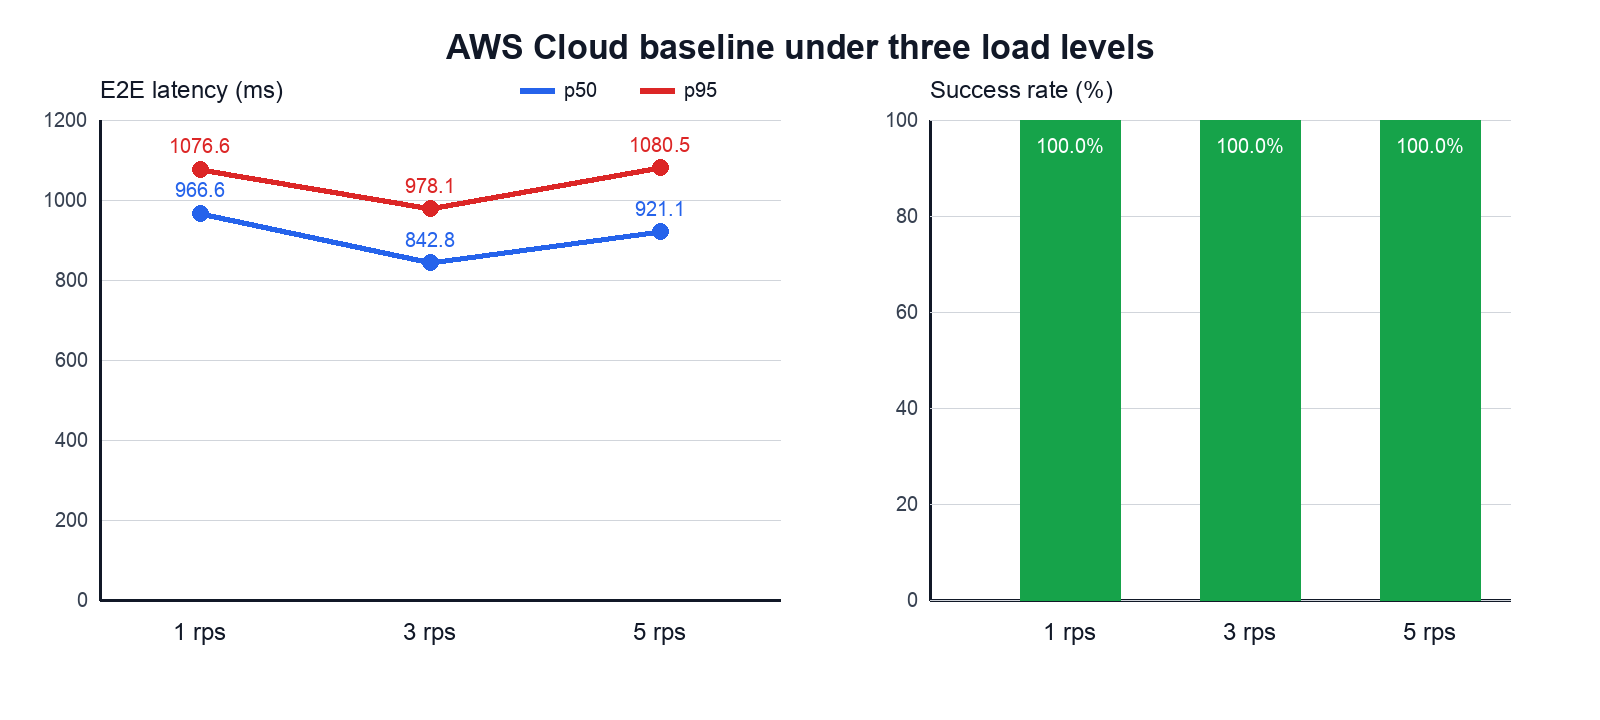
\includegraphics[width=\textwidth]{images/aws_yolo_load_latency.png}
    \caption{E2E latency và success rate của Lambda YOLOv8n theo tải}
    \label{fig:aws-load-results}
\end{figure}

Ở cả ba mức tải, hệ thống hoàn tất 100\% request và throughput quan sát bám sát tải
mục tiêu. p50 thấp nhất tại 3 request/s (842,85 ms) rồi tăng lên 921,08 ms tại
5 request/s; p95 lần lượt là 1076,56; 978,10 và 1080,49 ms. Vì mỗi cấu hình mới
chạy một lần, dao động này chỉ được mô tả, không được diễn giải thành quan hệ nhân
quả giữa tải và latency.

Tail latency vẫn xuất hiện: giá trị lớn nhất tăng từ 1293,42 ms lên 2451,32 ms khi
đạt 5 request/s, dù p95 chỉ quanh 1,08 giây. Do đã tách được thời gian suy luận,
các ngoại lệ E2E không thể quy hoàn toàn cho YOLO; chúng còn bao gồm API,
Step Functions scheduling, Lambda invocation và đọc S3.

Cold-start được đo riêng ngoài ma trận. Invocation đầu tiên sau deploy có E2E
64,41 giây, Detect 16,14 giây và inference đầu tiên 15,75 giây; CloudWatch ghi một
\texttt{INIT\_REPORT} chạm ngưỡng 10 giây. Invocation ấm kế tiếp giảm xuống E2E
1,97 giây, Detect 363,59 ms và inference 271,32 ms. Vì vậy năm invocation đồng
thời được dùng làm warm-up và không được tính vào 1620 request chính.

\paragraph{Phân rã stage, execution và Lambda Duration.}

Ngoài E2E, Detect phát \texttt{ModelInferenceLatency},
\texttt{ImageDownloadLatency} và \texttt{DetectLatency}; Alert phát
\texttt{AlertLatency}. CloudWatch Logs được ghép với CSV theo
\texttt{request\_id}, do đó bảng dưới dùng đúng 180/540/900 mẫu và không lẫn năm
warm-up. \texttt{Duration} được lấy từ dòng \texttt{REPORT} tương ứng của từng
invocation.

\begin{table}[htbp]
    \centering
    \caption{Phân rã metric CloudWatch theo ba mức tải}
    \label{tab:aws-cloudwatch-breakdown}
    \begin{tabular}{|l|r|r|r|}
        \hline
        \textbf{Metric} & \textbf{1 req/s} & \textbf{3 req/s}
        & \textbf{5 req/s} \\ \hline
        Detect stage trung bình (ms) & 357,104 & 244,440 & 289,559 \\ \hline
        YOLO inference trung bình (ms) & 306,660 & 194,452 & 240,028 \\ \hline
        Tải ảnh S3 trung bình (ms) & 49,765 & 49,357 & 48,874 \\ \hline
        Alert stage trung bình ($\mu$s) & 5,307 & 5,396 & 5,533 \\ \hline
        ExecutionsSucceeded & 180 & 540 & 900 \\ \hline
        ExecutionsFailed & 0 & 0 & 0 \\ \hline
        Lambda Detect Duration trung bình (ms) & 359,021 & 246,246 & 291,450 \\ \hline
        Lambda Alert Duration trung bình (ms) & 2,067 & 1,705 & 1,781 \\ \hline
    \end{tabular}
\end{table}

\begin{figure}[htbp]
    \centering
    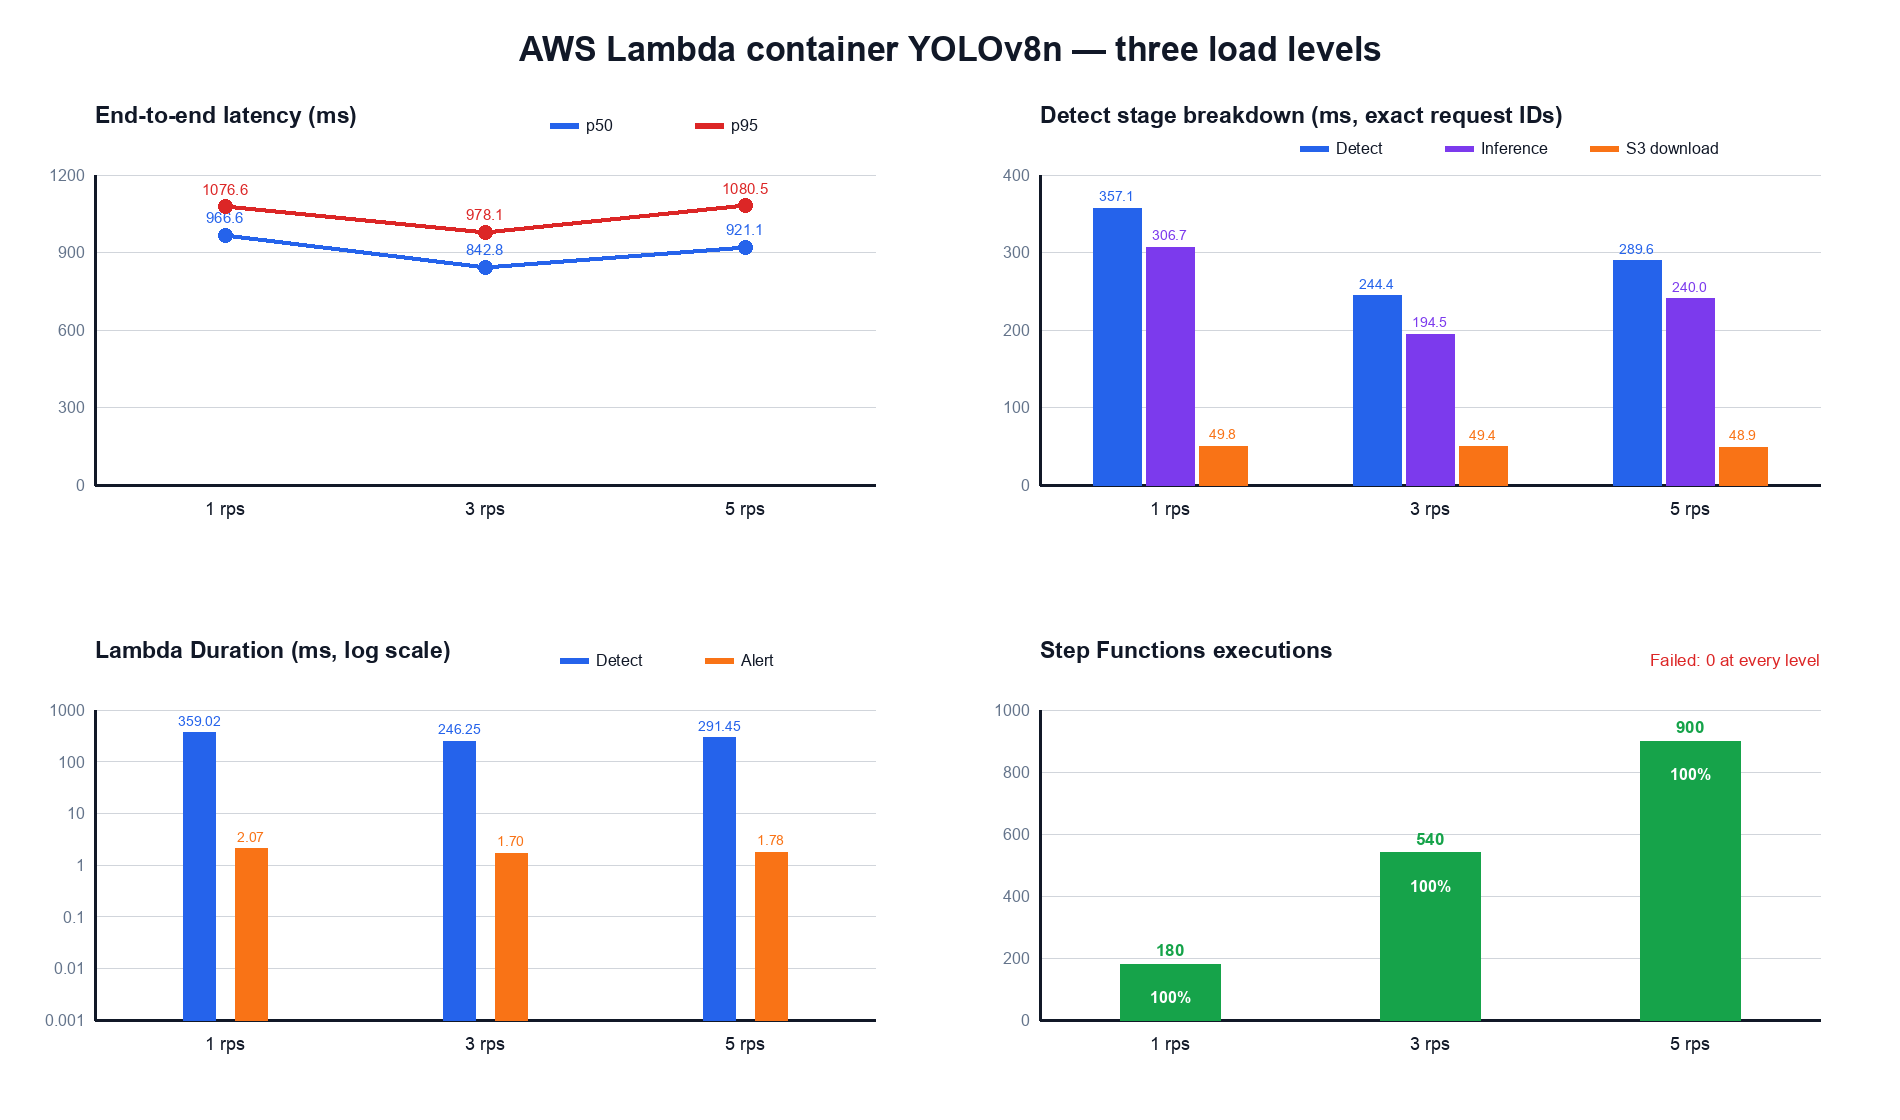
\includegraphics[width=0.98\linewidth,keepaspectratio]{images/aws_yolo_metrics.png}
    \caption{E2E, YOLO stage, Lambda Duration và execution theo tải}
    \label{fig:aws-cloudwatch-breakdown}
\end{figure}

YOLO inference chiếm phần lớn Detect stage: khoảng 306,66/357,10 ms ở 1 request/s,
194,45/244,44 ms ở 3 request/s và 240,03/289,56 ms ở 5 request/s. Tải ảnh S3 ổn
định quanh 49 ms; phần còn lại trong Detect chỉ khoảng 0,7--1,0 ms. Alert predicate
chỉ mất khoảng 5,3~$\mu$s nên đồ thị Lambda Duration dùng thang logarit để vẫn nhìn
thấy stage nhẹ này.

Lambda Detect Duration cao hơn timer Detect khoảng 1,9--2,2 ms, còn Lambda Alert
Duration nằm trong khoảng 1,705--2,067 ms. Chênh lệch phản ánh wrapper handler và
runtime ngoài đoạn code được gắn timer. Theo tài liệu AWS, Lambda
\texttt{Duration} không bao gồm toàn bộ cold-start initialization
\cite{awsLambdaMetrics}; cold-start vì thế được báo cáo bằng phép đo riêng.

Nếu định nghĩa một phần dư mô tả là

\begin{equation}
L_{\mathrm{residual}} = \overline{L}_{\mathrm{E2E}}
- \overline{D}_{\mathrm{Detect}} - \overline{D}_{\mathrm{Alert}},
\label{eq:cloud-residual}
\end{equation}

thì phần dư lần lượt là 607,07 ms, 608,72 ms và 632,32 ms. Đây không phải ``chi phí
Step Functions thuần túy'': nó còn gồm \texttt{StartExecution}, lập lịch dịch vụ,
chuyển trạng thái, Lambda invocation và các phần thời gian ngoài handler. Dù YOLO
là tải tính toán thật, khoảng 0,61--0,63 giây vẫn nằm ngoài Duration của hai hàm;
quan sát này trực tiếp củng cố động lực đo chi phí điều phối đầu cuối.

Số execution thành công trên CloudWatch khớp với CSV ở cả ba workload và không có
execution thất bại. Tuy nhiên, AWS mô tả metric Step Functions là best-effort và có
thể được phát theo ngữ nghĩa at-least-once \cite{awsStepFunctionsMetrics}. Vì vậy,
CSV và trạng thái execution vẫn là nguồn kiểm kê chính xác của thí nghiệm;
CloudWatch được dùng để quan sát xu hướng và kiểm tra chéo.

\paragraph{Mô phỏng có kiểm soát.}

\begin{table}[htbp]
    \centering
    \caption{Kết quả Cloud và Edge simulator theo ba mức tải}
    \label{tab:sim-results}
    \resizebox{0.98\linewidth}{!}{%
    \begin{tabular}{|l|r|r|r|r|r|r|}
        \hline
        \textbf{Chỉ số} & \multicolumn{2}{c|}{\textbf{1 req/s}}
        & \multicolumn{2}{c|}{\textbf{3 req/s}}
        & \multicolumn{2}{c|}{\textbf{5 req/s}} \\ \cline{2-7}
        & \textbf{Cloud} & \textbf{Edge} & \textbf{Cloud} & \textbf{Edge}
        & \textbf{Cloud} & \textbf{Edge} \\ \hline
        Số request & 180 & 180 & 540 & 540 & 900 & 900 \\ \hline
        Success rate & 100\% & 100\% & 100\% & 100\% & 100\% & 100\% \\ \hline
        Mean latency (ms) & 185,645 & 71,170 & 189,955 & 71,625
        & 172,497 & 68,637 \\ \hline
        p50 latency (ms) & 185,953 & 75,003 & 190,400 & 75,001
        & 170,510 & 67,515 \\ \hline
        p95 latency (ms) & 226,466 & 96,882 & 228,535 & 98,087
        & 213,872 & 94,718 \\ \hline
        p99 latency (ms) & 241,432 & 103,145 & 240,155 & 102,303
        & 243,307 & 98,256 \\ \hline
        Throughput (req/s) & 1,005 & 1,005 & 3,003 & 3,005
        & 5,002 & 5,005 \\ \hline
        Payload ngoài (MB) & 448,073 & 0 & 1344,219 & 0
        & 2240,365 & 0 \\ \hline
    \end{tabular}
    }
\end{table}

\begin{figure}[htbp]
    \centering
    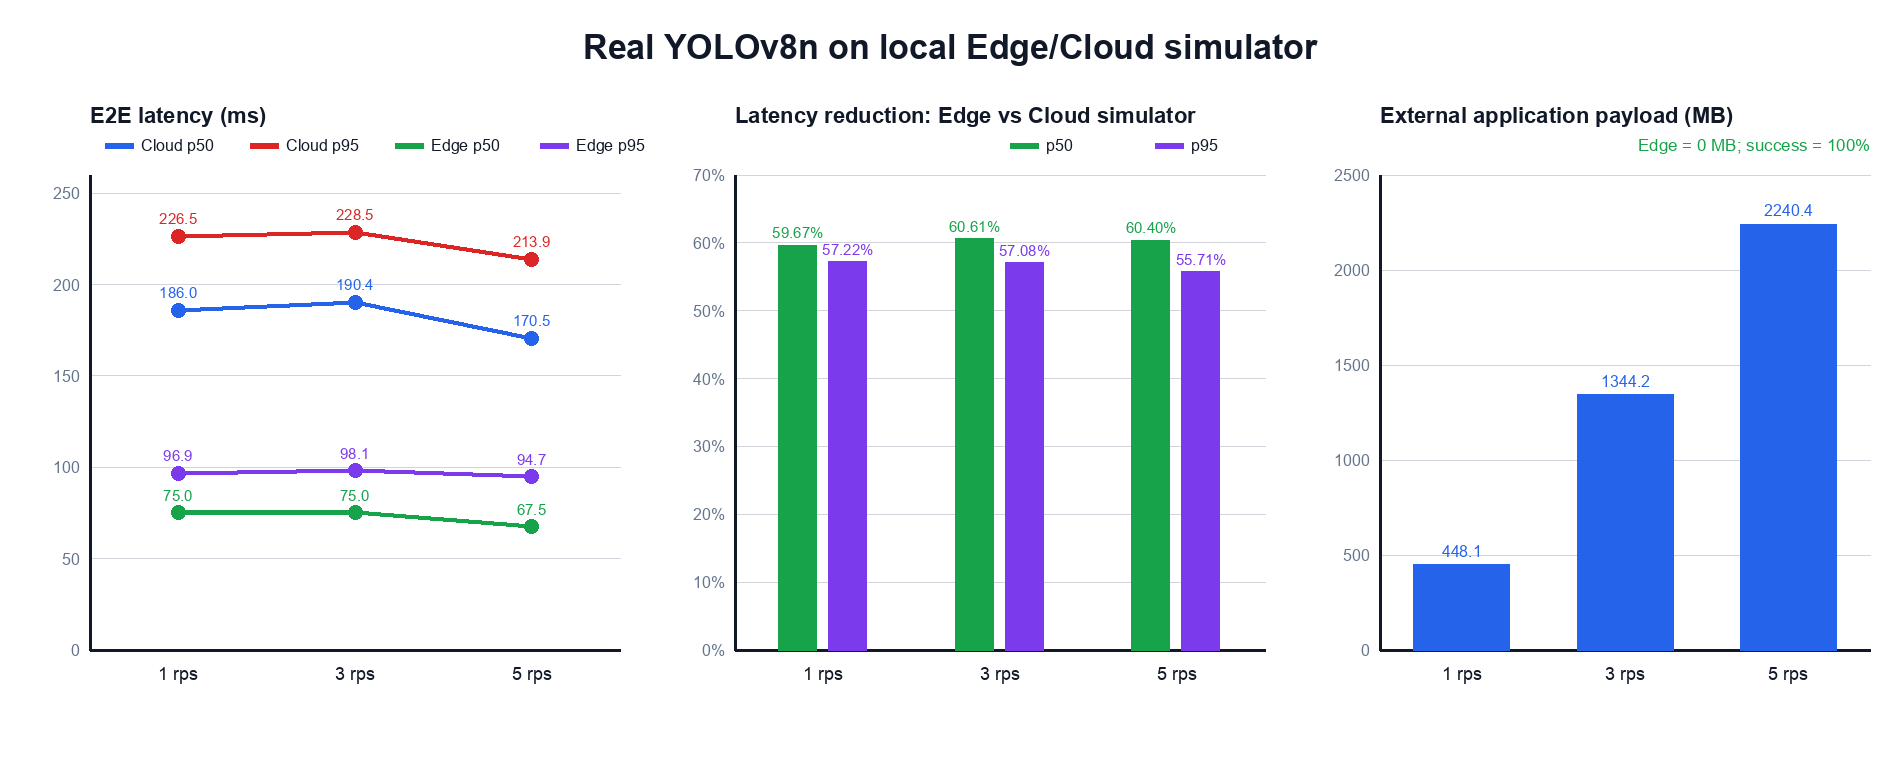
\includegraphics[width=\textwidth]{images/yolo_simulator_comparison.png}
    \caption{So sánh Cloud và Edge simulator khi cùng chạy YOLOv8n thật}
    \label{fig:yolo-simulator-results}
\end{figure}

Các cột latency có đơn vị ms, throughput có đơn vị request/s và payload dùng MB
thập phân ($1~\mathrm{MB}=10^6$ byte). p50 của Edge simulator thấp hơn Cloud
simulator 59,67\%, 60,61\% và 60,40\%; p95 giảm 57,22\%, 57,08\% và 55,71\%.
Hai nhánh dùng cùng YOLOv8n thật, cùng ảnh và warm-up, nên chênh lệch trong
simulator phản ánh các khoảng trễ uplink/transition/downlink được mô hình hóa cùng
đường chuyển trực tiếp trong tiến trình. Đây vẫn chưa phải latency IPC Greengrass.

Edge simulator không phát external application payload. Cloud simulator ghi nhận
448,073 MB, 1344,219 MB và 2240,365 MB vì mô hình đếm ảnh tuần tự hóa cùng payload
trả về qua đường biên Cloud. Giá trị tăng gần tuyến tính theo số request và tương
ứng khoảng 2,489 MB/request. Kết quả phù hợp với H2 trong mô hình dữ liệu đã định
nghĩa, nhưng không gồm TCP/IP, TLS và không phải số byte đo tại network interface
thật của Greengrass.

Cả sáu lần chạy đều đạt success rate 100\%. Throughput quan sát xấp xỉ đúng tốc độ
mục tiêu ở cả Cloud và Edge simulator, trong khi p50 và p95 chỉ biến động nhỏ. Vì
vậy, chưa quan sát thấy backlog hoặc bão hòa trong phạm vi 1--5 request/s. Mỗi cấu
hình mới được lặp một lần nên chênh lệch nhỏ giữa các rate chỉ được xem là mô tả,
không phải kết luận thống kê.

\begin{figure}[htbp]
    \centering
    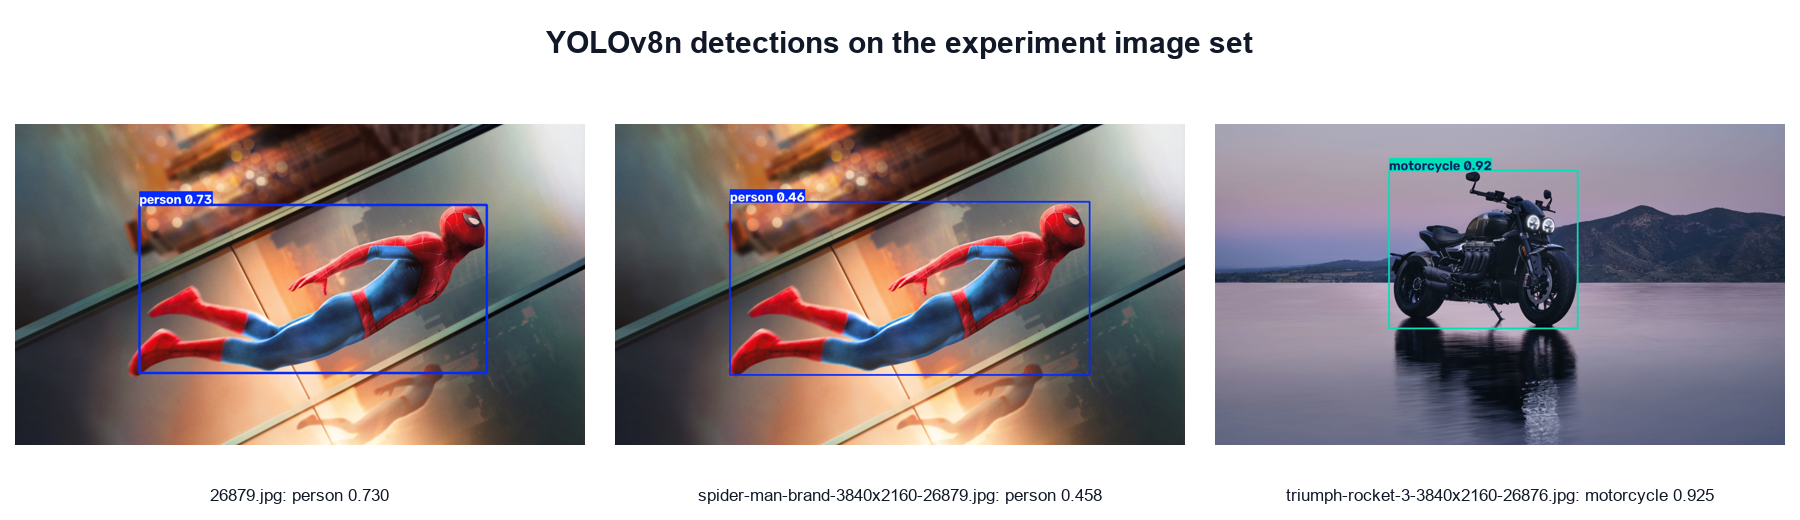
\includegraphics[width=\textwidth]{images/yolov8_detection_examples.png}
    \caption{Kết quả nhận diện YOLOv8n trên ba ảnh dùng trong workload}
    \label{fig:yolo-detection-examples}
\end{figure}

Hình~\ref{fig:yolo-detection-examples} xác nhận backend sinh kết quả thị giác thật:
hai ảnh Spider-Man được gán nhãn \texttt{person} với confidence 0,730 và 0,458;
ảnh xe được gán \texttt{motorcycle} với confidence 0,925. Chỉ detection
\texttt{person} có confidence ít nhất 0,60 kích hoạt cảnh báo, vì vậy mỗi chu kỳ ba
ảnh có một cảnh báo xâm nhập. Tổng cộng AWS ghi 540 cảnh báo trên 1620 request.

\subsection{Thảo luận và đối chiếu giả thuyết}

\paragraph{Nguyên tắc đối chiếu.}
Bài báo của Malazi và cộng sự là nghiên cứu kiến trúc và không công bố một bộ số
liệu p50, p95, throughput hoặc network byte làm đường chuẩn
\cite{malazi2026orchestrating}. Vì vậy, không thể tính hệ số tương quan thống kê hay
so sánh trực tiếp giá trị latency của demo với ``chỉ số của bài báo''. Cách đối
chiếu phù hợp là chuyển các luận điểm của bài báo thành các đại lượng quan sát được:

\begin{itemize}
    \item BA6 và IC4 được lượng hóa bằng external payload và E2E latency;
    \item BA7 được lượng hóa bằng p50, p95 và khoảng cách giữa các percentile;
    \item BA9 và IC7 cần completion rate trong điều kiện mất kết nối;
    \item resource feasibility cần CPU, RAM và năng lượng.
\end{itemize}

\paragraph{Tương quan giữa luận điểm và kết quả.}
Kết quả simulator phù hợp với hướng dự đoán của BA6 và BA7: khi đường truy cập
state và handoff được rút ngắn, latency và external payload cùng giảm. Mức giảm p50
nằm trong khoảng 59,67--60,61\%. Với workload 5 request/s, mức giảm p95 được minh
họa như sau:

\begin{equation}
G_{p95}^{(5)} = \frac{213{,}872 - 94{,}718}{213{,}872}\times 100\%
= 55{,}71\%.
\label{eq:p95-reduction}
\end{equation}

External payload giảm từ khoảng 2,489 MB/request xuống 0 trong mô hình simulator.
Hai kết quả này cung cấp bằng chứng ban đầu phù hợp với BA6, BA7 và IC4, nhưng
không xác nhận mức cải thiện trên Greengrass thật.

Với Cloud baseline thật, 1620/1620 execution thành công xác nhận workflow có thể
vận hành và thu telemetry ở ba mức tải. Tỷ số $p95/p50$ lần lượt xấp xỉ 1,114;
1,160 và 1,173 ở 1, 3 và 5 request/s. Giá trị lớn nhất tại 5 request/s đạt
2451,32 ms, cho thấy tail latency vẫn cần theo dõi dù p95 chỉ 1080,49 ms. Số liệu không
cho phép quy phần đuôi này riêng cho Step Functions vì E2E còn bao gồm API call,
S3, Lambda scheduling và cold start.

Phép phân rã CloudWatch Logs bổ sung một quan sát phù hợp với động lực của BA7:
tổng Duration trung bình của hai Lambda nằm trong khoảng 247,95--361,09 ms, trong
khi E2E trung bình ở mức 856,67--968,15 ms. Phần dư ổn định quanh 607--632 ms cho
thấy tối ưu riêng YOLO chưa đủ để tối ưu toàn chuỗi. Tuy vậy, phần dư E2E chỉ
là chỉ báo tổng hợp về các chi phí ngoài handler, không phải phép đo trực tiếp chi
phí handoff của riêng Step Functions.

\begin{table}[htbp]
    \centering
    \caption{Đối chiếu luận điểm bài báo với các chỉ số và kết quả thực nghiệm}
    \label{tab:paper-result-correlation}
    \begin{tabular}{|p{2.1cm}|p{3.2cm}|p{4.2cm}|p{4.1cm}|}
        \hline
        \textbf{Luận điểm} & \textbf{Chỉ số đại diện} & \textbf{Kết quả quan sát}
        & \textbf{Mức độ hỗ trợ} \\ \hline

        BA6, IC4 & External payload; E2E latency & Payload simulator giảm khoảng
        2,489 MB/request xuống 0; Edge simulator có p50 thấp hơn & Phù hợp với hướng
        dự đoán trong mô phỏng; chưa đo network interface Greengrass \\ \hline

        BA7 & p50, p95; chi phí handoff & p50 giảm 59,67--60,61\%; p95 giảm
        55,71--57,22\%
        trong simulator & Ủng hộ composition-aware co-location trong mô phỏng;
        chưa phải số đo IPC thật \\ \hline

        BA9, IC7 & Completion rate khi mất uplink & Chưa có thí nghiệm ngắt kết
        nối & Chưa đánh giá \\ \hline

        Resource feasibility & CPU, peak RSS, năng lượng & Chưa có dữ liệu trên
        thiết bị Edge & Chưa đánh giá \\ \hline

        Telemetry agent & Success rate; p50; p95; stage và Duration & AWS:
        1620/1620 thành công; YOLO inference 194,45--306,66 ms; phần dư ngoài hai
        Lambda 607--632 ms & Xác nhận khả năng phân rã Cloud baseline;
        không phải bằng chứng so sánh Edge \\ \hline
    \end{tabular}
\end{table}

Bảng~\ref{tab:paper-result-correlation} cho thấy mức độ bao phủ của thực nghiệm:
BA6 và BA7 đã có bằng chứng mô phỏng; BA9, IC7 và resource feasibility mới dừng ở
mức định hướng. Do đó, tương quan được báo cáo là tương quan về \emph{hướng tác
động} và mức độ bao phủ luận điểm, không phải tương quan thống kê giữa hai bộ dữ
liệu.

\begin{table}[htbp]
    \centering
    \caption{Trạng thái đánh giá các giả thuyết}
    \label{tab:hypotheses}
    \begin{tabular}{|p{1.5cm}|p{5cm}|p{7cm}|}
        \hline
        \textbf{Giả thuyết} & \textbf{Trạng thái} & \textbf{Căn cứ} \\ \hline
        H1 & Được ủng hộ trong mô phỏng & p50 và p95 Edge simulator thấp hơn
        Cloud simulator; chưa có Greengrass benchmark \\ \hline
        H2 & Được ủng hộ trong mô hình payload & Edge simulator không phát
        external payload; chưa đo network interface thật \\ \hline
        Khả năng offline & Chưa kiểm chứng & Chưa thực hiện thí nghiệm ngắt uplink
        trên Greengrass Core \\ \hline
        Đánh đổi CPU/RAM & Chưa kiểm chứng & Chưa có telemetry tài nguyên trên thiết
        bị Edge \\ \hline
    \end{tabular}
\end{table}


\section{Hạn chế và kế hoạch hoàn thiện}

\subsection{Hạn chế}

Kết quả hiện tại chịu năm giới hạn chính. Thứ nhất, YOLOv8n đã chạy thật nhưng tập
ba ảnh không có nhãn nên không đánh giá accuracy hoặc mAP. Thứ hai, Edge path vẫn
là mô phỏng trong tiến trình Python, chưa bao gồm Greengrass IPC và giới hạn tài
nguyên của thiết bị. Thứ ba, AWS và simulator không phải hai môi trường tương
đương. Thứ tư, mỗi mức tải mới chạy một lần. Cuối cùng, network byte mới được đếm
ở tầng ứng dụng trong simulator, chưa đo tại network interface Greengrass.

Do các giới hạn này, báo cáo không đưa ra kết luận rằng Greengrass thực tế giảm
55--61\% latency. Khoảng giảm 59,67--60,61\% ở p50 và 55,71--57,22\% ở p95 chỉ
mô tả simulator YOLOv8n hiện tại.

\subsection{Kế hoạch thực nghiệm Greengrass}

Để trả lời đầy đủ câu hỏi nghiên cứu, cần thực hiện các bước sau:

\begin{enumerate}
    \item Cài Greengrass Core V2 trên một VM Linux có cấu hình CPU/RAM cố định.
    \item Triển khai Detect và Alert dưới dạng hai component pinned; Detect gọi
    Alert qua IPC cục bộ.
    \item Dùng cùng model YOLOv8n, tập ảnh, ngưỡng confidence và logic Alert cho
    cả Cloud và Edge.
    \item Warm-up 10 request; chạy các mức 1, 5, 10 và 20 request/s; ít nhất 100
    request mỗi mức và lặp năm lần.
    \item Đo p50, p95, p99, throughput, success rate, byte tại network interface,
    CPU và peak RSS.
    \item Chạy riêng thí nghiệm ngắt uplink để đánh giá khả năng hoàn tất workflow
    cục bộ; không trộn dữ liệu này với benchmark mạng bình thường.
\end{enumerate}

Kết quả cuối cần báo cáo median và IQR của các lần lặp. Chỉ khi Cloud và Edge dùng
cùng workload và quy trình đo mới có thể tính mức giảm latency thực nghiệm.


\section{Kết luận}

Nghiên cứu đã xây dựng và kiểm chứng chức năng của Cloud baseline gồm S3, Step
Functions, Lambda Detect, Lambda Alert và CloudWatch. Ba workload 1, 3 và 5
request/s hoàn tất 1620/1620 execution. p50 nằm trong khoảng 842,85--966,56 ms và
p95 nằm trong khoảng 978,10--1080,49 ms. Cụ thể, p50 là 966,56; 842,85 và
921,08 ms ở 1, 3 và 5 request/s. Hệ thống chưa có dấu hiệu bão hòa theo success
rate, nhưng giá trị lớn nhất 2451,32 ms tại 5 request/s cho thấy vẫn tồn tại đuôi
dài.

CloudWatch Logs ghép theo request ID cho thấy YOLO inference trung bình
194,45--306,66 ms, Detect stage 244,44--357,10 ms và tải ảnh S3 gần 49 ms. Tổng
Lambda Duration của hai hàm là 247,95--361,09 ms, còn phần dư ngoài hai handler
ổn định quanh 607--632 ms. Khoảng cách này xác nhận sự cần thiết phải đánh giá toàn
đường xử lý thay vì chỉ đo thời gian mô hình, nhưng chưa cô lập chi phí riêng của
Step Functions.

Trong môi trường mô phỏng có kiểm soát, đường gọi cục bộ đạt p50 thấp hơn
59,67--60,61\%, p95 thấp hơn 55,71--57,22\% và không phát external application
payload. Quan sát này ủng hộ giả thuyết được rút
ra từ BA6, BA7 và IC4 rằng data locality và giảm handoff có thể cải thiện chuỗi hàm
\cite{malazi2026orchestrating}. Tuy nhiên, Edge simulator không thay thế cho
Greengrass benchmark.

Đóng góp chính của đề tài ở giai đoạn hiện tại là một Lambda container YOLOv8n
thật có telemetry theo stage, một Cloud baseline 1620 request và một đối chứng
simulator dùng cùng model. Việc triển khai Greengrass với cùng model và ma trận tải
là điều kiện cần thiết để đưa ra kết luận định lượng cuối cùng về hiệu quả của hệ
thống.
